\section{NegBioDB: A Database of Negative Results}
\label{sec:database}

NegBioDB is a multi-domain database of experimentally confirmed negative results in biomedicine, aggregating 32.9M entries from 12 data sources across three domains. We first describe the common design principles, then detail each domain.

\subsection{Design Principles}

All three domains share a common abstraction layer: each record encodes a \emph{hypothesis} (e.g., ``compound X inhibits target Y''), \emph{experimental evidence} (assay type, method, publication), an \emph{outcome} (inactive, failed, non-interacting), and a \emph{confidence tier} reflecting evidence quality. The four-tier system is:
\textbf{Gold}---systematic screens or multiple independent confirmations (e.g., DAVIS kinase panel, HuRI Y2H screen);
\textbf{Silver}---single quantitative measurement or statistical evidence (e.g., $p>0.05$ from clinical trial, ML-derived from co-purification data);
\textbf{Bronze}---computationally derived or NLP-detected (e.g., STRING zero-score pairs, NLP-classified trial terminations);
\textbf{Copper}---label-only annotations without detailed evidence.
Table~\ref{tab:overview} summarizes the database scope.

\begin{table}[t]
\centering
\caption{NegBioDB database overview across three biomedical domains.}
\label{tab:overview}
\small
\begin{tabular}{@{}lrrrr@{}}
\toprule
 & \textbf{DTI} & \textbf{CT} & \textbf{PPI} & \textbf{Total} \\
\midrule
Negative results     & 30.5M   & 132,925  & 2.23M   & 32.9M \\
Key entities         & 919K / 3.7K & 177K / 56K & 18.4K & --- \\
                     & \scriptsize{(cpd / tgt)} & \scriptsize{(interv / cond)} & \scriptsize{(proteins)} & \\
Data sources         & 4       & 4        & 4       & 12 \\
Confidence tiers     & 3       & 4        & 3       & 4 \\
DB size              & 13.2 GB & 0.5 GB   & 0.8 GB  & 14.6 GB \\
\midrule
ML benchmark runs    & 18      & 108      & 54      & 180 \\
LLM benchmark runs   & 81      & 80       & 80      & 241 \\
\bottomrule
\end{tabular}
\end{table}

\subsection{Three Domains}

\textbf{Drug--Target Interaction (DTI).}
We aggregate inactive compound--target pairs from four sources: ChEMBL~\citep{gaulton2017chembl} bioactivity records with pChEMBL $<5$ (i.e., IC$_{50}$ $>10\,\mu$M); PubChem~\citep{kim2023pubchem} confirmatory inactives from dose-response screens; BindingDB~\citep{gilson2016bindingdb} entries with $K_d > 10\,\mu$M; and the full DAVIS kinase selectivity matrix~\citep{davis2011comprehensive}, where untested pairs are excluded. This yields 30.5M negative results across 919K compounds and 3,694 targets---three orders of magnitude larger than standard DTI benchmarks that rely on assumed negatives~\citep{huang2021therapeutics,mysinger2012dude}.

\textbf{Clinical Trial Failure (CT).}
We process 216,987 trials from the AACT database~\citep{tasneem2012aact} through a three-tier failure detection pipeline: (i)~NLP classification of termination reasons into 7 failure categories (bronze tier); (ii)~statistical evidence extraction from outcome measures where $p>0.05$ indicates non-superiority (silver/gold tiers); and (iii)~integration of the Clinical Trial Outcome dataset~\citep{siah2021cto} for label-only records (copper tier). Drug names are resolved to ChEMBL identifiers through a four-step cascade (exact match, PubChem API, fuzzy matching with Jaro--Winkler $>0.90$, manual curation), achieving 20.6\% resolution with SMILES structures. The pipeline identifies 132,925 failure results with 8 failure categories: safety, efficacy, enrollment, strategic, regulatory, design, pharmacokinetic, and other.

\textbf{Protein--Protein Interaction (PPI).}
We compile confirmed non-interactions from four sources spanning different evidence types: IntAct~\citep{orchard2014intact} curated non-interactions from co-immunoprecipitation and two-hybrid assays (779 gold/silver pairs); HuRI~\citep{luck2020huri} systematic yeast two-hybrid screen negatives sampled from 39.9M candidates via reservoir sampling (500K gold pairs); hu.MAP~\citep{drew2021humap} ML-derived non-interactions from co-purification mass spectrometry (1.23M silver pairs); and STRING~\citep{szklarczyk2023string} zero-score pairs between well-studied proteins (500K bronze pairs). After cross-source aggregation, NegBioDB contains 2.23M unique negative PPI pairs across 18,412 human proteins with UniProt-validated identifiers and sequences (99.6\% coverage).

\begin{figure}[t]
\centering
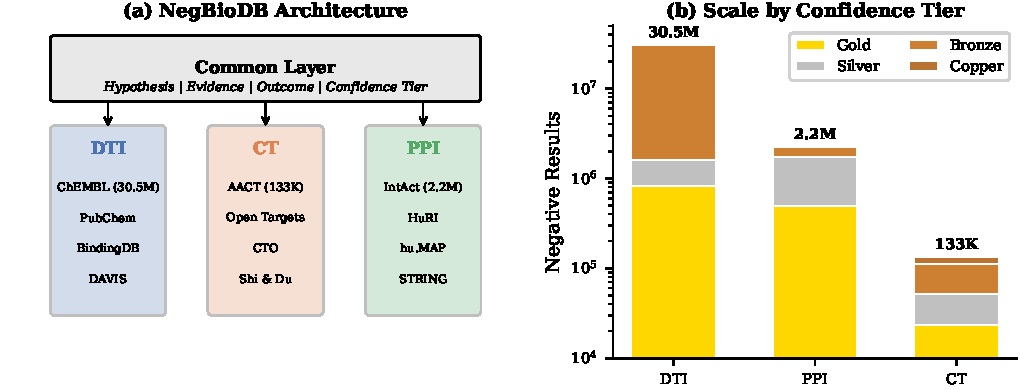
\includegraphics[width=\textwidth]{figures/fig1_overview.pdf}
\caption{NegBioDB overview. \textbf{(a)} Architecture showing three domains unified by a common abstraction layer with four confidence tiers. Each domain integrates four data sources. \textbf{(b)} Scale of negative results by domain and confidence tier (log scale). DTI dominates in volume (30.5M), while CT and PPI contribute qualitatively distinct evidence types.}
\label{fig:overview}
\end{figure}
